\chapter{Instrukcja użytkownika}
\label{chapter:5}

Interfejs aplikacji jest podzielony na 4 sekcje, zaznaczony na rysunku \ref{fig:interface}.

\begin{enumerate}
    \item Widok stołu: w tym miejscu użytkownik może zaznaczyć kursorem miejsce na karty gracza, wspólne, bądź ,,martwe", wyjęte z talii na czas obliczeń. Po procesie kalkulacji pojawiają się tu także szanse na zwycięstwo graczy biorących udział w rozdaniu.
    \item Menu kart: po wybraniu karta zostaje umieszczona w miejscu zaznaczonym przez kursor.
    \item Przycisk reset: służący do resetu widoku oraz otrzymanych wyników
    \item Sekcja wyników: zawiera liczbę kombinacji oraz tabelę z szansami na poszczególne układy dla każdego z graczy
\end{enumerate}

\begin{figure}[ht]
    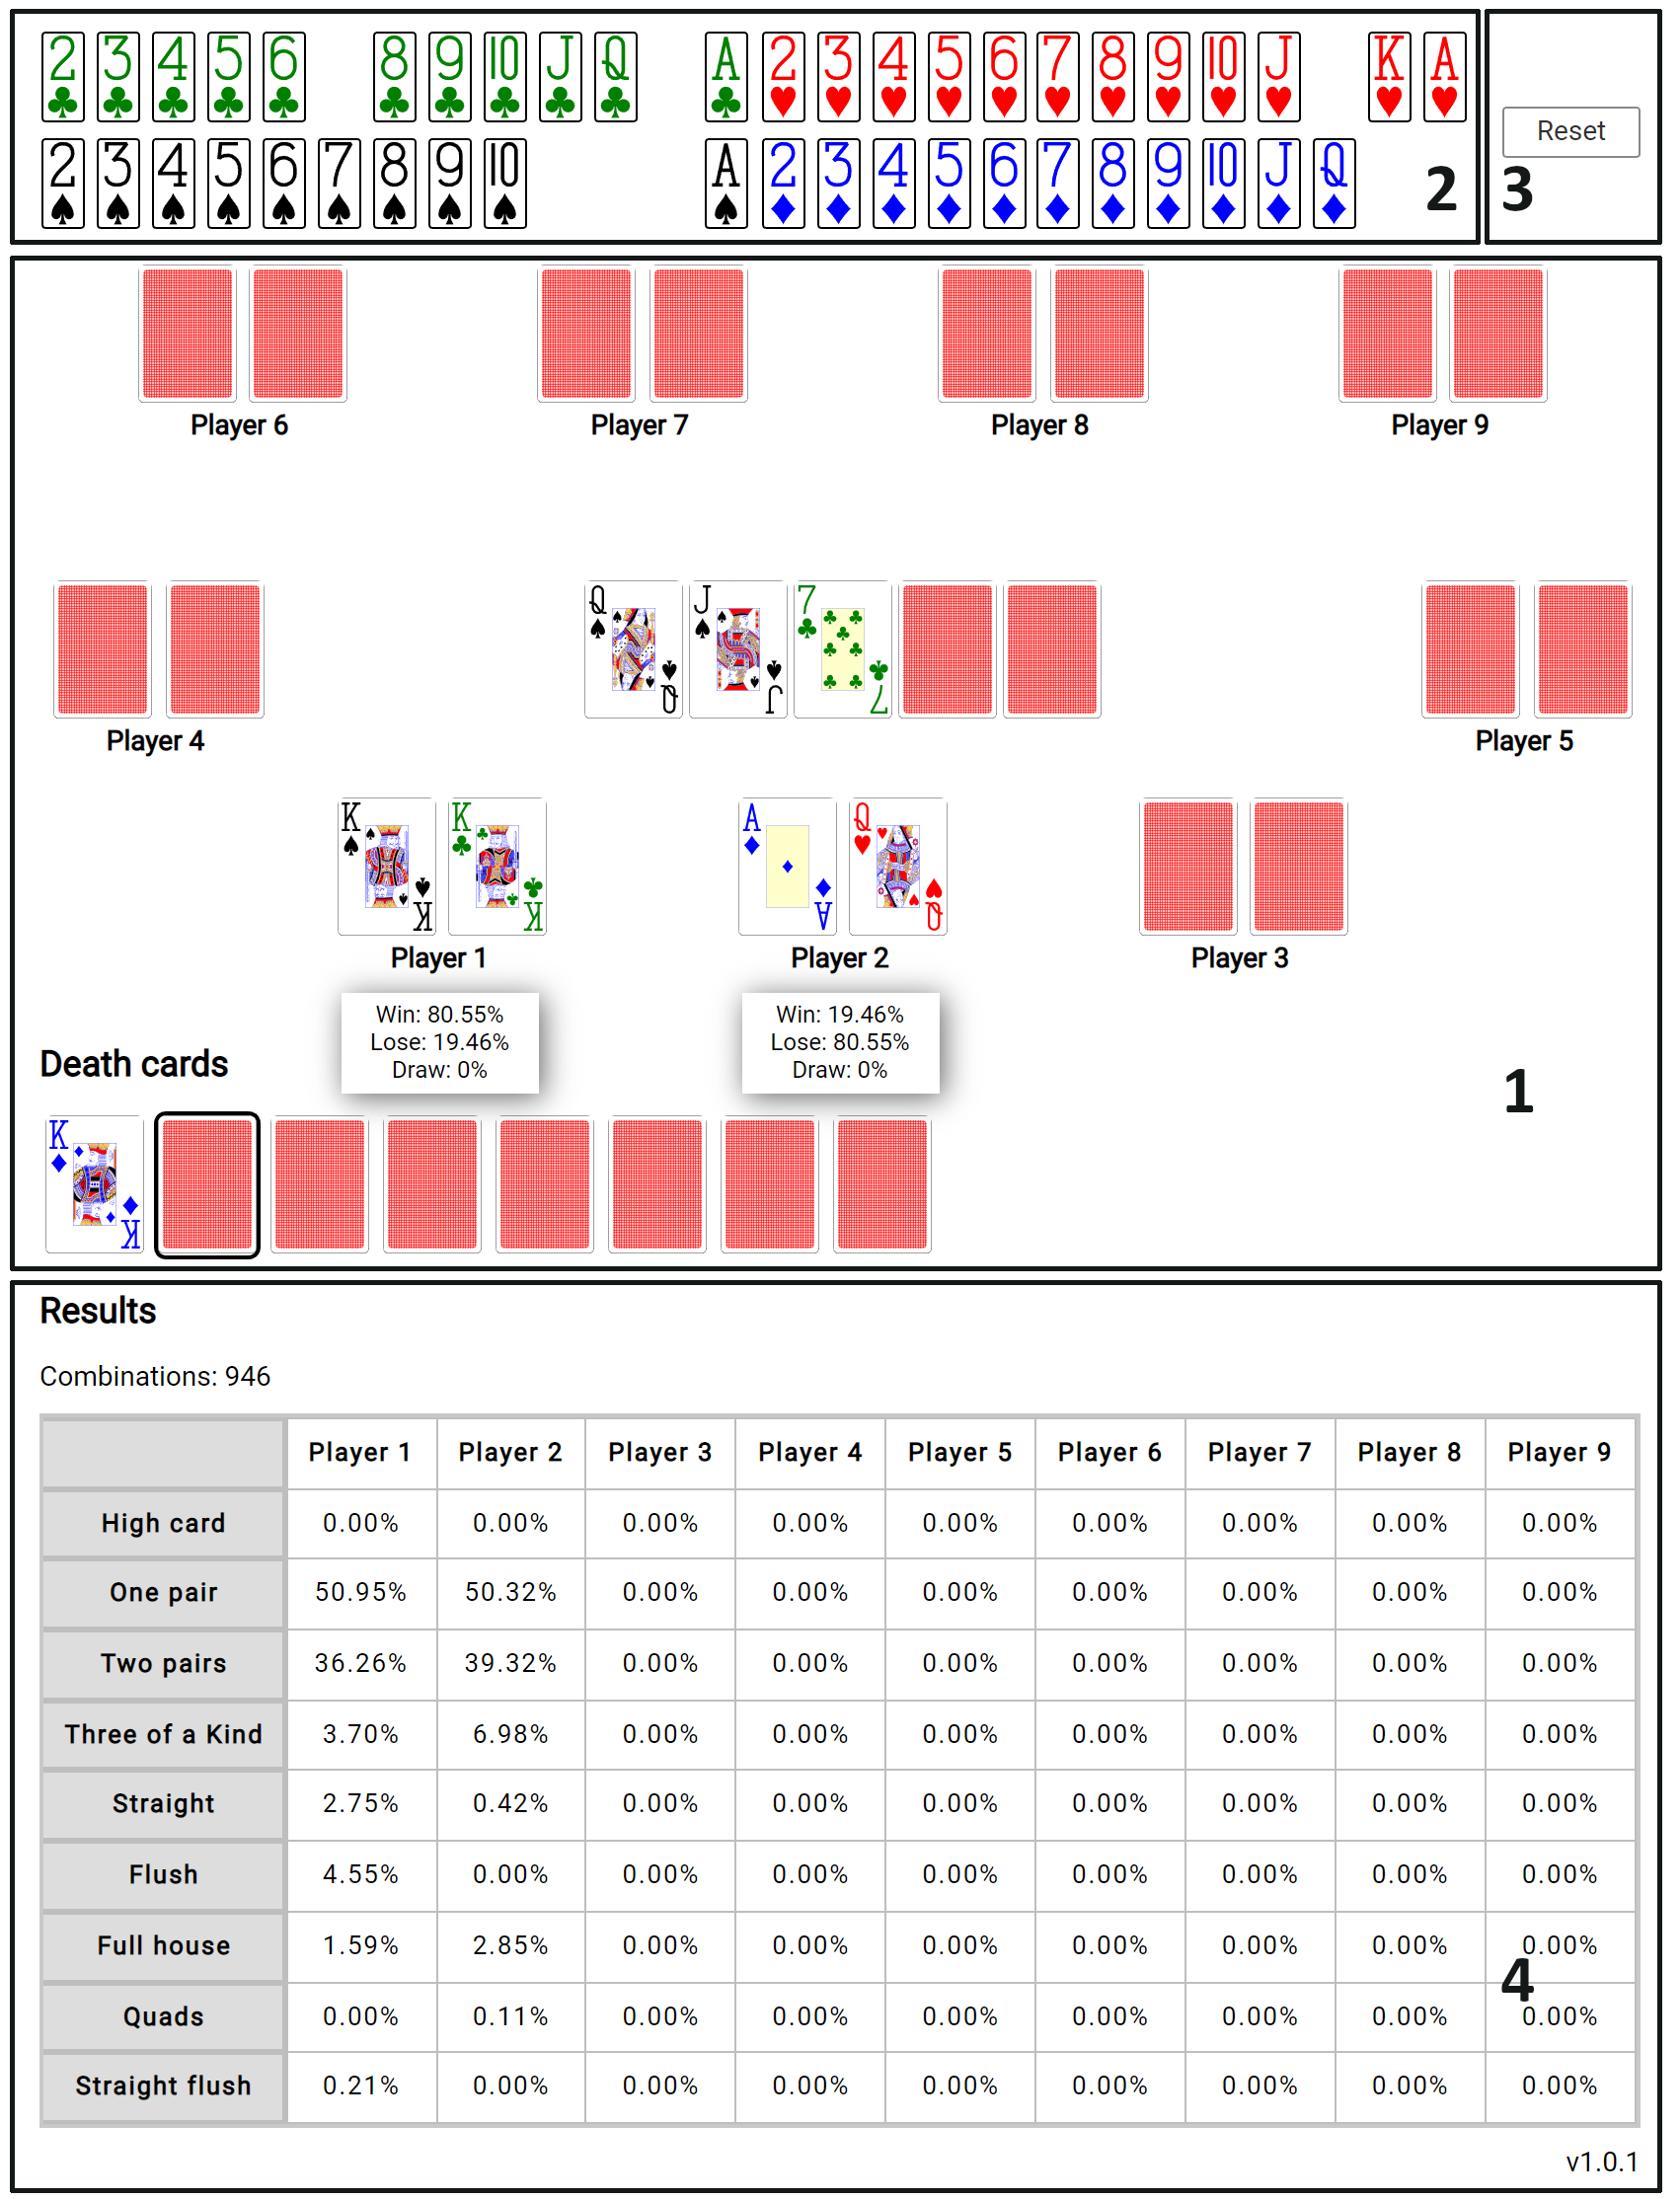
\includegraphics[width=\textwidth]{images/interface.png}
    \caption{Interfejs użytkownika z kolejno zaznaczonymi sekcjami}
    \label{fig:interface}
\end{figure}

Użytkownik zaznacza poszczególne elementy interfejsu lewym przyciskiem myszy, bądź korzystając z klawisza Enter. Dodatkowo interfejs umożliwia nawigację po wszystkich elementach korzystając z klawiszy Tab oraz Tab+Shift. Poza przyciskiem do resetu scenariusza można usuwać pojedyncze karty lewym przyciskiem myszy lub klawiszem Enter. Po umieszczeniu karty nie trzeba kolejny raz wybierać miejsca docelowego --- kursor aplikacji przemieszcza się z kolejnymi wyborami kart.
